\section{V5}
\subsection{Data Alignment}
\begin{minipage}{6cm}   
    \begin{tabular}{|l|l|l|}
        \hline 
        1 Byte & 8 Bit  & Byte  \\ 
        \hline 
        2 Byte & 16 Bit & Half-Word \\ 
        \hline 
        4 Byte & 32 Bit & Word \\ 
        \hline 
        8 Byte & 64 Bit & Double-Word \\ 
        \hline 
    \end{tabular} 
\end{minipage}
\begin{minipage}{12cm}
    \subsubsection{Aligned-Unaligned Data}
    \begin{multicols}{2}
            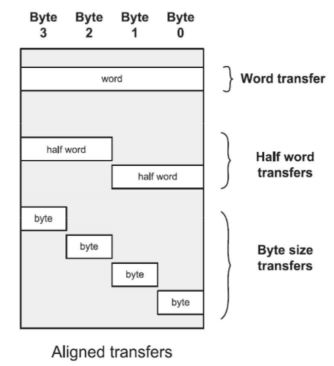
\includegraphics[width=0.5\textwidth]{images/alignedData}
            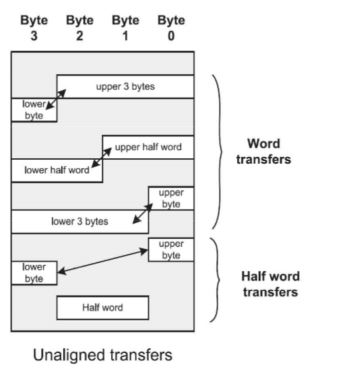
\includegraphics[width=0.5\textwidth]{images/unalignedData}
    \end{multicols}
\end{minipage}
\subsubsection{Bit-Banding}
\vspace{-0.5cm}
\[\textbf{ BitBandAliasAddress = BitBandAliasBase + (MemoryAddres - BitbandRegionBase)* 32 + 4*BitNumber} \]
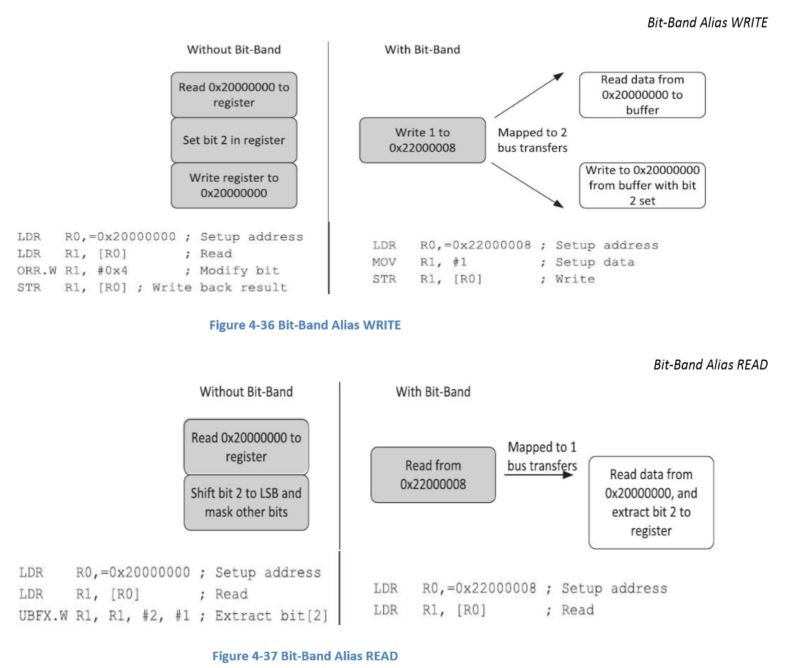
\includegraphics[width=0.85\textwidth]{images/bitbanding}